\section{Week 1 - Notes: Introduction to Classical
Mechanics}\label{week-1---notes-introduction-to-classical-mechanics}

\subsection{How do we formulate Classical
Mechanics?}\label{how-do-we-formulate-classical-mechanics}

In the past, you have learned about
\href{https://en.wikipedia.org/wiki/Newton\%27s_laws_of_motion}{Newton's
Laws of Motion}. These laws are the foundation of classical mechanics.
They are used to describe the motion of objects in the universe. In this
course, we will use these laws to describe the motion of particles and
rigid bodies. As we progress, we will learn other formulations of
classical mechanics, such as the
\href{https://en.wikipedia.org/wiki/Lagrangian_mechanics}{Lagrangian}
and
\href{https://en.wikipedia.org/wiki/Hamiltonian_mechanics}{Hamiltonian}
reformulations.

Newton's Laws of Motion are a vector formulation of classical mechanics.
The laws are as follows: 1. \textbf{First Law}: An object at rest will
remain at rest, and an object in motion will remain in motion at a
constant velocity unless acted upon by an external force. 2.
\textbf{Second Law}: The acceleration of an object is directly
proportional to the net force acting on it and inversely proportional to
its mass. The direction of the acceleration is in the direction of the
net force. 3. \textbf{Third Law}: For every action, there is an equal
and opposite reaction.

These are the classic laws of motion that you have learned in other
courses. How we formulate these laws mathematically is the subject of
this course.

\subsection{Newton's Second Law}\label{newtons-second-law}

\href{https://en.wikipedia.org/wiki/Newton\%27s_laws_of_motion\#Newton's_second_law}{Newton's
Second Law} provides the mathematical foundation for classical
mechanics. It provides a vector relationship between the net force
acting on an object and its acceleration. The law is given by the
equation:

\[\vec{F}_{net} = m\vec{a}\]

where \(\vec{F}_{net}\) is the net force acting on the object, \(m\) is
the mass of the object, and \(\vec{a}\) is the acceleration of the
object. This equation is a vector equation, meaning that it must be
satisfied in each direction.

\[\begin{aligned}
F_{net,x} &= m a_x \\
F_{net,y} &= m a_y \\
F_{net,z} &= m a_z
\end{aligned}\]

Each push in a Cartesian direction results in a proportional response --
an acceleration in the same direction of the net push. Let's go through
a common example to illustrate this relationship.

\subsubsection{Example: A Block on an Inclined
Ramp}\label{example-a-block-on-an-inclined-ramp}

Consider the box (mass, \(m\)) above on an inclined ramp (angle,
\(\theta\)). The box is at rest subject to static friction, \(\mu_s\).
\emph{What angle of inclination will cause the box to start sliding down
the ramp?}

We start by drawing the
\href{https://en.wikipedia.org/wiki/Free_body_diagram}{Free Body
Diagram} (FBD) of the box.

\pandocbounded{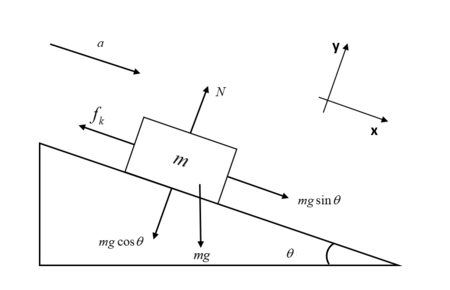
\includegraphics[keepaspectratio,alt={Free Body Diagram of Box on a Inclined Ramp; the arrows label the direction of forces acting on the box}]{../images/notes/week1/box_fbd.png}}
\href{images/notes/week1/diagram_2_450x3002352212273710292.png}{Source:
homework.study.com}

The FBD is a diagram that shows all the forces acting on the object. In
this case, the forces acting on the box are: - The force of gravity,
\(mg\), acting downwards. - The force due to the ramp, which is both
perpendicular to the ramp surface (normal) and parallel to it
(friction).

We tilt our coordinate system to align with the ramp. This makes the
normal force, \(N\), act in the \(y\)-direction and the frictional
force, \(f\), act in the \(x\)-direction. The force of gravity is split
into two components: \(mg\sin(\theta)\) and \(mg\cos(\theta)\).

The net force acting on the box is the sum of the forces acting on it,
and is zero up to the point where the box starts sliding. At this point,
the frictional force is at its maximum value, \(\mu_s N\). Taking the
sum of the forces acting on the box in each direction we have:

\[\vec{F}_{net} = \vec{f} + \vec{N} + \vec{F}_{gravity} = 0\]

\[\sum F_{x,i} = f - mg\sin(\theta) = 0\]
\[\sum F_{y,i} = N - mg\cos(\theta) = 0\]

Thus,

\[f = mg\sin(\theta)\] \[N = mg\cos(\theta)\]

At the point where the box starts sliding, the frictional force is at
its maximum value, \(\mu_s N\). Thus, the box starts sliding when:

\[f = \mu_s N\]

Substituting the expressions for \(f\) and \(N\) into the equation
above, we have:

\[mg\sin(\theta) = \mu_s mg\cos(\theta)\]

Solving for \(\theta\):

\[\tan(\theta) = \mu_s\] \[\theta = \tan^{-1}(\mu_s)\]

Thus, the box starts sliding when the angle of inclination is equal to
the arctangent of the coefficient of static friction.

```\{admonition\} Check We can check this with some numbers. Steel as a
static friction coefficient of about 0.16, and rubber is closer to 0.8.
Thus, the angle of inclinations for steel and rubber are:

\[\theta_{steel} = \tan^{-1}(0.16) \approx 9^\circ\]
\[\theta_{rubber} = \tan^{-1}(0.8) \approx 39^\circ\]

It seems quite reasonable that rubber would have a higher angle of
inclination before sliding than steel.

\begin{verbatim}
```{tip}
A few things to note about this problem:
1. This was a static problem, such that $\vec{F}_{net} = 0$.
2. We rotated our coordinate system to align with the ramp. This is a common technique in classical mechanics to simplify the problem.
3. We still used Cartesian coordinates to solve the problem. This is because the forces could be easily decomposed in the titled coordinate system.
\end{verbatim}

Let's work an example that is dynamic, where the net force is not zero.

\subsubsection{Example: Falling Object in One
Dimension}\label{example-falling-object-in-one-dimension}

Consider an object of mass \(m\) falling, but it is subject to air
resistance. The free body diagram of the object shows that the forces
acting on the object are: - The force of gravity/weight, \(W=mg\),
acting downwards. - The force due to air resistance, \(F_{air}\), acting
upwards.

\pandocbounded{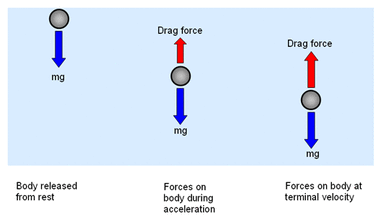
\includegraphics[keepaspectratio,alt={Free Body Diagram of Falling Object; the arrows label the direction of forces acting on the object}]{../images/notes/week1/falling_object.png}}
\href{images/notes/week1/570899611.gif}{Source:
ibphysicsguide.weebly.com}

Here we have chosen positive \(y\) to be the downward direction. We want
to predict the motion (\(a\), \(v\), \(y\)) of the object as a function
of time. This is a very common problem for classical mechanics.

\paragraph{Air Drag?}\label{air-drag}

First, we notice that we do not know the force due to
\href{https://en.wikipedia.org/wiki/Drag_(physics)}{air resistance}. We
do know that the force is related to the velocity of the object. So
let's start by writing the air resistance force as a function of
velocity:

\[F_{air} = F(v)\]

where \(F(v)\) is some function of velocity.

\paragraph{Taylor Series Expansion}\label{taylor-series-expansion}

Because we know that the objects move slowly in classical mechanics, we
can assume that the function can be expanded using a
\href{https://en.wikipedia.org/wiki/Taylor_series}{Taylor Series}. In
general, the Taylor Series of a function \(f(x)\) about a point \(a\) is
given by:

\[f(x) = \sum_{n=0}^{\infty} \frac{f^{(n)}(a)}{n!}(x-a)^n\]

where \(f^{(n)}(a)\) is the \(n\)-th derivative of \(f(x)\) evaluated at
\(x=a\). We can write the first few terms out,

\[f(x) = f(a) + f'(a)(x-a) + \frac{f''(a)}{2!}(x-a)^2 + \frac{f'''(a)}{3!}(x-a)^3 + \ldots\]

Because we know that the object is moving slowly, we can expand the
function \(F(v)\) about \(v=0\):

\[F(v) = F(0) + F'(0)v + \frac{F''(0)}{2!}v^2 + \ldots\]

We can assume that the first term is zero, \(F(0)=0\), because there is
no air resistance when the object is at rest. Thus, the force due to air
resistance is approximately:

\[F(v) \approx F'(0)v + \frac{F''(0)}{2!}v^2\]

We call the first term the \textbf{linear drag} term and the second term
the \textbf{quadratic drag} term. The linear drag term is proportional
to the velocity of the object, and the quadratic drag term is
proportional to the square of the velocity of the object. We also
typically replace the evaluated derivatives with constants, \(b\) and
\(c\) -- because they are constants that depend on the object and the
fluid it is moving through. And thus,

\[F_{air} \approx bv + cv^2\]

\paragraph{Back to Newton's Second
Law}\label{back-to-newtons-second-law}

In the \(y\)-direction, the net force acting on the object is:

\[F_y = W - F_{air} = mg - bv - cv^2\]

And thus, the acceleration of the object is:

\[a = g - \frac{b}{m}v - \frac{c}{m}v^2\]

This
\href{(https://en.wikipedia.org/wiki/Differential_equation)}{differential
equation} can be written in a variety of ways. One common way is to
write the equation as a
\href{https://math.libretexts.org/Bookshelves/Differential_Equations/Introduction_to_Partial_Differential_Equations_(Herman)/12:_B_-_Ordinary_Differential_Equations_Review/12.02:_Second_Order_Linear_Differential_Equations}{second-order
differential equation}.

\[\frac{d^2y}{dt^2} = g - \frac{b}{m}\frac{dy}{dt} - \frac{c}{m}\left(\frac{dy}{dt}\right)^2\]

Note that this is a nonlinear differential equation (i.e., there's a
\((d^ny/dt^n)^m\) term where \(m > 1\)), which are notoriously difficult
to solve in general. We can write it using the dot notation for
derivatives (i.e., \(\dot{y} = dy/dt\), \(\ddot{y} = d^2y/dt^2\)):

\[\ddot{y} = g - \frac{b}{m}\dot{y} - \frac{c}{m}\dot{y}^2\]

We can also use the velocity as the independent variable,
\(v = \dot{y}\). Both equations below are equivalent:

\[\frac{dv}{dt} = g - \frac{b}{m}v - \frac{c}{m}v^2\]
\[\dot{v} = g - \frac{b}{m}v - \frac{c}{m}v^2\]

\texttt{\{tip\}\ A\ few\ things\ to\ note:\ 1.\ This\ is\ a\ dynamic\ one-dimensional\ problem,\ such\ that\ \$\textbackslash{}vec\{F\}\_\{net\}\ \textbackslash{}neq\ 0\$.\ 2.\ This\ is\ a\ nonlinear\ problem,\ such\ that\ the\ acceleration\ is\ a\ function\ of\ the\ velocity\ of\ the\ object.\ 3.\ We\ are\ stuck\ with\ a\ differential\ equation\ that\ we\ need\ to\ solve,\ and\ don\textquotesingle{}t\ have\ a\ simple\ algebraic\ solution\ (e.g.,\ a\ simple\ antiderivative).}

\textbf{How do we solve this equation to find the motion of the object
as a function of time?} We will come back to this, but solving
differential equations is the primary tool of classical mechanics. We
will learn how to solve these equations analytically and numerically in
this course.
